\documentclass[final,3p,times,12pt]{article}
\usepackage[utf8]{inputenc}
\usepackage{graphicx, float} 
\graphicspath{{images/}}
\usepackage{amsmath, amssymb, amsthm}
\usepackage{subcaption}
\usepackage[title,titletoc]{appendix}
\usepackage[utf8]{inputenc} % Required for inputting international characters
\usepackage[T1]{fontenc} % Output font encoding for international characters
\usepackage{graphicx}
\usepackage{enumitem}
\usepackage{longtable}
\usepackage{stmaryrd}
%\usepackage{mathpazo} % Palatino font
\usepackage[colorlinks=true, linkcolor=black, citecolor=black, urlcolor=black]{hyperref}
\usepackage{array}
\usepackage[svgnames]{xcolor}
% Define the dark green color
\definecolor{darkgreen}{rgb}{0.0, 0.5, 0.0} % Adjust RGB values as needed
% Setting margin sizes
\usepackage[letterpaper, top=1.0in, bottom=1.0in, left=1.0in, right=1.0in, heightrounded]{geometry}
% Line height
\renewcommand{\baselinestretch}{1.15} % linespacing
% Parskip and Parindent (sets the space between paragraphs)
\setlength{\parskip}{0.8em}
\usepackage{tocloft}
\setlength{\cftbeforesecskip}{5pt}
\setlength{\cftbeforesubsecskip}{5pt}
\setlength{\cftbeforesubsubsecskip}{5pt}
\usepackage{caption}  % For captions under figures
\bibliographystyle{ieeetr}
\usepackage{listings}
\usepackage{color}
\usepackage{booktabs}


% Define the style for Python code
\lstdefinestyle{pythoncode}{
  language=Python,
  basicstyle=\scriptsize,
  keywordstyle=\color{blue},
  commentstyle=\color{darkgreen},
  stringstyle=\color{red},
  showstringspaces=false,
  identifierstyle=\color{black},
  procnamekeys={def,class},
  frame=single, % adds a frame around the code
  rulecolor=\color{black}, % if not set, the frame-color may be changed on line-breaks within not-black text
  breaklines=true, % sets automatic line breaking
  captionpos=b, % sets the caption-position to bottom
  numbers=left, % where to put the line-numbers
  numberstyle=\tiny\color{black}, % the style that is used for the line-numbers
  numbersep=10pt, % how far the line-numbers are from the code
  tabsize=4, % sets default tabsize to 2 spaces
}
\lstset{style=pythoncode}

\begin{document}

\begin{titlepage}
    \centering
    \vspace*{2cm}
    
    {\Large \textbf{COMP0078}}\\[1cm] % Module Code
    {\Huge \textbf{Supervised Learning Coursework 2}}\\[1cm] % Title
    
    \vspace{1cm}
    
    {\Large December 2024}\\[1.5cm] % Date
    
    % Optional additional information, like your name or university
    {\Large University College London} % Replace with your university name if applicable
    
    \vfill
    
    % Optional logo placement (if desired)
    % \includegraphics[width=0.3\textwidth]{path_to_your_logo.png}
    
    \vspace{2cm}
    
\end{titlepage}
\newpage

\tableofcontents
\newpage


\section{Part 1 - Rademacher Complexity of finite Spaces}

\subsection{} We have : \[
\bar{X} = \lambda .\frac{1}{\lambda}.\bar{X} = \frac{1}{\lambda}.log(e^{\lambda.\bar{X}})
\]
\[
\implies E(\bar{X}) = E(\frac{1}{\lambda}.log(e^{\lambda.\bar{X}}))\]
\[
\implies E(\bar{X}) = \frac{1}{\lambda}.E(log(e^{\lambda.\bar{X}}))\]

$e^{\lambda.\bar{X}}$ is positive, and the log function is concave. We can therefore use Jensen's inequality to obtain:  
\[
E(\bar{X}) \leq \frac{1}{\lambda}.log(E(e^{\lambda.\bar{X}}))
\]\\

\subsection{} If we write $l=\arg\max_i (X_i)$, we have : 
\[
e^{\bar{X}} = e^{X_l} \leq  e^{X_l} + \sum_{i=1, i\neq l}^m e^{X_i} = \sum_{i=1}^m e^{X_i} \]

\[
\implies  e^{\lambda\bar{X}} \leq \sum_{i=1}^m e^{\lambda X_i} \]\\

If we remind that $\forall i \in \{1,\dots,m\}, E(X_i) = 0$, and if we use the given hint, we obtain that : 
\[
\sum_{i=1}^m e^{\lambda X_i} = \sum_{i=1}^m e^{\lambda(X_i - E(X_i))} \leq \sum_{i=1}^m e^{\frac{\lambda^2(b-a)^2}{8}} = m.e^{\frac{\lambda^2(b-a)^2}{8}}\]

\[ \implies \frac{1}{\lambda}.log(E(e^{\lambda\bar{X}})) \leq \frac{1}{\lambda}.log(E(m.e^{\frac{\lambda^2(b-a)^2}{8}})) = \frac{1}{\lambda}.log(m.e^{\frac{\lambda^2(b-a)^2}{8}}) = \frac{1}{\lambda}.log(m) +  \frac{\lambda(b-a)^2}{8}\]\\

We finally obtain the demanded inequality : 

\[ \frac{1}{\lambda}.log(E(e^{\lambda\bar{X}})) \leq \frac{1}{\lambda}.log(m) +  \frac{\lambda(b-a)^2}{8}\]\\

\subsection{} Let's fix $\lambda = \frac{2.\sqrt{2.log(m)}}{b-a}$. We use the inequality from question 2 to obtain :  

\[ E(\bar{X}) \leq \frac{1}{\lambda}.log(m) + \lambda.\frac{(b-a)^2}{8}\]
\[ \implies E(\bar{X}) \leq \frac{(b-a).log(m)}{2.\sqrt{2.log(m)}} + \frac{2.\sqrt{2.log(m)}}{b-a}.\frac{(b-a)^2}{8}\]
\[ \implies E(\bar{X}) \leq \frac{(b-a).\sqrt{2.log(m)}}{2.\sqrt{2}.\sqrt{2}} + \frac{(b-a).\sqrt{2.log(m)}}{4}\]
\[ \implies E(\bar{X}) \leq \frac{(b-a).\sqrt{2.log(m)}}{2} \]

We have demonstrated the demanded inequality : $E(\bar{X}) \leq \frac{(b-a).\sqrt{2.log(m)}}{2}$ \\

Note : to obtain the value of $\lambda$, we proceeded as follows.\\

First, we noticed that $\lambda$ had to satisfy the inequality : 

\[\frac{(b-a).\sqrt{2.log(m)}}{2} \geq \frac{1}{\lambda}.log(m) +  \frac{\lambda(b-a)^2}{8}\]

This inequality is equivalent to : 
\[
0 \geq log(m) +  \frac{\lambda^2(b-a)^2}{8} - \frac{(b-a).\sqrt{2.log(m)}}{2}.\lambda
\]

We then compute the discriminant $\Delta$ of this inequality : 
\[
\Delta = \frac{(b-a)^2.2.log(m)}{4} - 4.\frac{(b-a)^2}{8}.log(m) = 0
\]

This inequality only admits one solution : $\lambda = \frac{(b-a).\sqrt{2.log(m)}}{2}.\frac{8}{2.(b-a)^2} = \frac{2.\sqrt{2.log(m)}}{(b-a)}$

\subsection{} 

First, for any a > 0, we can define . Let's first apply Jensen's inequality f(E(X)) $\leq$ E(f(X)) to the function f defined by f(x) : x $\rightarrow$ $e^{ax}$ for any a > 0, and X = $\max_{x\in S} \frac{1}{n}.\sum_{j=1}^n \sigma_j.x_j$ : 

\[
e^{a.\mathbb{E}_{\sigma}\left(\max_{x\in S} \frac{1}{n}.\sum_{j=1}^n \sigma_j.x_j\right)} \leq \mathbb{E}_{\sigma}\left(e^{a.\max_{x\in S} (\frac{1}{n}.\sum_{j=1}^n \sigma_j.x_j)}\right)
\]

\[ \implies
e^{a.\mathbb{E}_{\sigma}\left(\max_{x\in S} \frac{1}{n}.\sum_{j=1}^n \sigma_j.x_j\right)} \leq \mathbb{E}_{\sigma}\left(\max_{x\in S}e^{a.\frac{1}{n}.\sum_{j=1}^n \sigma_j.x_j}\right)
\]

\[ \implies
e^{a.\mathbb{E}_{\sigma}\left(\max_{x\in S} \frac{1}{n}.\sum_{j=1}^n \sigma_j.x_j\right)} \leq \sum_{x\in S}\mathbb{E}_{\sigma}\left(e^{a.\frac{1}{n}.\sum_{j=1}^n \sigma_j.x_j}\right)
\] \\

$\forall (i,i') \in \{1, ...,n\}^2$, $\sigma_i$ and  $\sigma_i'$ are iid, therefore : 

\[
e^{a.\mathbb{E}_{\sigma}\left(\max_{x\in S} \frac{1}{n}.\sum_{j=1}^n \sigma_j.x_j\right)} \leq  \sum_{x\in S}\prod_{j=1}^n\mathbb{E}_{\sigma}\left(e^{a.\frac{1}{n}. \sigma_j.x_j}\right)
\] \\

Since $\forall j \{1, ..., n\}, \sigma_j.x_j \in \{-x_j,x_j\}$, we have that $\mathbb{E}_{\sigma}\left(a.\frac{1}{n}. \sigma_j.x_j\right) = 0$. Therefore, we can use Hoeffding’s Lemma : 

\[
e^{a.\mathbb{E}_{\sigma}\left(\max_{x\in S} \frac{1}{n}.\sum_{j=1}^n \sigma_j.x_j\right)} \leq  \sum_{x\in S}\prod_{j=1}^n\mathbb{E}_{\sigma}\left(e^{a.\frac{1}{n}. \sigma_j.x_j}\right) \leq \sum_{x\in S}\prod_{j=1}^n e^{a^2.\frac{1}{n^2}. 4.x_j^2.\frac{1}{8}} = \sum_{x\in S}\prod_{j=1}^n e^{\frac{a^2}{2.n^2}.x_j^2.}
\] \\

\[ \implies
e^{a.\mathbb{E}_{\sigma}\left(\max_{x\in S} \frac{1}{n}.\sum_{j=1}^n \sigma_j.x_j\right)} \leq \sum_{x\in S} e^{\frac{a^2}{2.n^2}.\sum_{j=1}^nx_j^2} = \sum_{x\in S} e^{\frac{a^2}{2.n^2}.||x||_2^2} \leq m.\max_{x\in S}\left(e^{\frac{a^2}{2.n^2}.||x||_2^2}\right)
\] \\

\[ \implies
a.\mathbb{E}_{\sigma}\left(\max_{x\in S} \frac{1}{n}.\sum_{j=1}^n \sigma_j.x_j\right) \leq log(m)+\max_{x\in S}\left(\frac{a^2}{2.n^2}.||x||_2^2\right)
\] \\

\[ \implies
\mathbb{E}_{\sigma}\left(\max_{x\in S} \frac{1}{n}.\sum_{j=1}^n \sigma_j.x_j\right) \leq \frac{log(m)}{a}+ \max_{x\in S}(\frac{a}{2.n^2}.||x||_2^2) = \max_{x\in S}(\frac{a}{2.n^2}.||x||_2^2 + \frac{log(m)}{a})
\] \\

We then find the value $a_*$ minimizing our upper bound :

\[
\frac{\partial}{\partial a} \left( \frac{a.||x||_2^2}{2.n^2} + \frac{\log(m)}{a}\right) = 0
\]

\[ \implies
\frac{||x||_2^2}{2.n^2} -\frac{\log(m)}{a_*^2}  = 0
\]
\[ \implies
a_*^2 \frac{||x||_2^2}{2.n^2} = \log(m)
\]
\[ \implies
a_* = \frac{n}{||x||_2} \sqrt{2 \log(m)}
\]\\

Our upper bound now becomes : 

\[
\mathbb{E}_{\sigma}\left(\max_{x\in S} \frac{1}{n}.\sum_{j=1}^n \sigma_j.x_j\right) \leq \max_{x\in S}\left(\frac{a_*}{2.n^2}.||x||_2^2 + \frac{log(m)}{a_*}\right) = \max_{x\in S}\left(\frac{\sqrt{\log(m)}.||x||_2}{\sqrt{2}.n} + \frac{\sqrt{\log(m)}.||x||_2}{\sqrt{2}.n}\right)
\]

If we simplify the last term of our previous inequality, we obtain the demanded result : 

\[
\mathbb{E}_{\sigma}\left(\max_{x\in S} \frac{1}{n}.\sum_{j=1}^n \sigma_j.x_j\right) \leq \max_{x\in S}\left(\||x||_2\right)\frac{\sqrt{2.\log(m)}}{n}
\]

\subsection{} 

We have : $ R_{\mathcal{S}}(\mathcal{H}) = \sup_{f\in \mathcal{H}}\left(\frac{1}{n}.\sum_{j=1}^n \sigma_j.f(x_j)\right)$. We use the exact same reasoning as in question 4, and we fix m = $|\mathcal{H}|$ : 

First, for any a > 0, we can define . Let's first apply Jensen's inequality f(E(X)) $\leq$ E(f(X)) to the function f defined by f(x) : x $\rightarrow$ $e^{ax}$ for any a > 0, and X = $\sup_{f\in \mathcal{H}} \frac{1}{n}.\sum_{j=1}^n \sigma_j.f(x_j)$ : 

\[
e^{a.\mathbb{E}_{\sigma}\left(\sup_{f\in \mathcal{H}} \frac{1}{n}.\sum_{j=1}^n \sigma_j.f(x_j)\right)} \leq \mathbb{E}_{\sigma}\left(e^{a.\sup_{f\in \mathcal{H}} \left(\frac{1}{n}.\sum_{j=1}^n \sigma_j.f(x_j))\right)}\right)
\]

\[ \implies
e^{a.\mathbb{E}_{\sigma}\left(\sup_{f\in \mathcal{H}} \frac{1}{n}.\sum_{j=1}^n \sigma_j.f(x_j)\right)} \leq \mathbb{E}_{\sigma}\left(\sup_{f\in \mathcal{H}}e^{a.\frac{1}{n}.\sum_{j=1}^n \sigma_j.f(x_j)}\right)
\]

\[ \implies
e^{a.\mathbb{E}_{\sigma}\left(\sup_{f\in \mathcal{H}} \frac{1}{n}.\sum_{j=1}^n \sigma_j.f(x_j)\right)} \leq \sum_{x\in S}\mathbb{E}_{\sigma}\left(e^{a.\frac{1}{n}.\sum_{j=1}^n \sigma_j.f(x_j)}\right)
\] \\

$\forall (i,i') \in \{1, ...,n\}^2$, $\sigma_i$ and  $\sigma_i'$ are iid, therefore : 

\[
e^{a.\mathbb{E}_{\sigma}\left(\sup_{f\in \mathcal{H}} \frac{1}{n}.\sum_{j=1}^n \sigma_j.f(x_j)\right)} \leq  \sum_{x\in S}\prod_{j=1}^n\mathbb{E}_{\sigma}\left(e^{a.\frac{1}{n}. \sigma_j.f(x_j)}\right)
\] \\

Since $\forall j \{1, ..., n\}, \sigma_j.f(x_j) \in \{-f(x_j),f(x_j)\}$, we have that $\mathbb{E}_{\sigma}\left(a.\frac{1}{n}. \sigma_j.f(x_j)\right) = 0$. Therefore, we can use Hoeffding’s Lemma : 

\[
e^{a.\mathbb{E}_{\sigma}\left(\sup_{f\in \mathcal{H}} \frac{1}{n}.\sum_{j=1}^n \sigma_j.f(x_j)\right)} \leq  \sum_{x\in S}\prod_{j=1}^n\mathbb{E}_{\sigma}\left(e^{a.\frac{1}{n}. \sigma_j.f(x_j)}\right) \leq \sum_{x\in S}\prod_{j=1}^n e^{a^2.\frac{1}{n^2}. 4.f(x_j)^2.\frac{1}{8}} = \sum_{x\in S}\prod_{j=1}^n e^{\frac{a^2}{2.n^2}.f(x_j)^2.}
\] \\

\[ \implies
e^{a.\mathbb{E}_{\sigma}\left(\sup_{f\in \mathcal{H}} \frac{1}{n}.\sum_{j=1}^n \sigma_j.f(x_j)\right)} \leq \sum_{x\in S} e^{\frac{a^2}{2.n^2}.\sum_{j=1}^nf(x_j)^2} \leq m.\sup_{f\in \mathcal{H}}\left(e^{\frac{a^2}{2.n^2}.\sum_{j=1}^nf(x_j)^2}\right)
\] \\

\[ \implies
a.\mathbb{E}_{\sigma}\left(\sup_{f\in \mathcal{H}} \frac{1}{n}.\sum_{j=1}^n \sigma_j.f(x_j)\right) \leq log(m)+\sup_{f\in \mathcal{H}}\left(\frac{a^2}{2.n^2}.\sum_{j=1}^nf(x_j)^2\right)
\] \\

\[ \implies
\mathbb{E}_{\sigma}\left(\sup_{f\in \mathcal{H}} \frac{1}{n}.\sum_{j=1}^n \sigma_j.f(x_j)\right) \leq \frac{log(m)}{a}+ \sup_{f\in \mathcal{H}}(\frac{a}{2.n^2}.\sum_{j=1}^nf(x_j)^2) = \sup_{f\in \mathcal{H}}(\frac{a}{2.n^2}.\sum_{j=1}^nf(x_j)^2 + \frac{log(m)}{a})
\] \\

We then find the value $a_*$ minimizing our upper bound :

\[
\frac{\partial}{\partial a} \left( \frac{a.\sum_{j=1}^nf(x_j)^2}{2.n^2} + \frac{\log(m)}{a}\right) = 0
\]

\[ \implies
\frac{\sum_{j=1}^nf(x_j)^2}{2.n^2} -\frac{\log(m)}{a_*^2}  = 0
\]
\[ \implies
a_*^2 \frac{\sum_{j=1}^nf(x_j)^2}{2.n^2} = \log(m)
\]
\[ \implies
a_* = \frac{n}{\sqrt{\sum_{j=1}^nf(x_j)^2}} \sqrt{2 \log(m)}
\]\\

Our upper bound now becomes : 

\[
\mathbb{E}_{\sigma}\left(\sup_{f\in \mathcal{H}} \frac{1}{n}.\sum_{j=1}^n \sigma_j.f(x_j)\right) \leq \sup_{f\in \mathcal{H}}\left(\frac{a_*}{2.n^2}.\sum_{j=1}^nf(x_j)^2 + \frac{log(m)}{a_*}\right)
\]

\[ \implies
\mathbb{E}_{\sigma}\left(\sup_{f\in \mathcal{H}} \frac{1}{n}.\sum_{j=1}^n \sigma_j.f(x_j)\right) \leq \sup_{f\in \mathcal{H}}\left(\frac{\sqrt{\log(m)}.\sqrt{\sum_{j=1}^nf(x_j)^2}}{\sqrt{2}.n} + \frac{\sqrt{\log(m)}.\sqrt{\sum_{j=1}^nf(x_j)^2}}{\sqrt{2}.n}\right)
\]

If we simplify the last term of our previous inequality, we obtain the demanded result : 

\[
\mathbb{E}_{\sigma}\left(\sup_{f\in \mathcal{H}} \frac{1}{n}.\sum_{j=1}^n \sigma_j.f(x_j)\right) \leq \sup_{f\in \mathcal{H}}\left(\sqrt{\sum_{j=1}^nf(x_j)^2}\right)\frac{\sqrt{2.\log(m)}.}{n}
\]





   
\section{Part 2 - Bayes Decision Rule and Surrogate Approaches
}

\subsection{}

We can write : 
\[
R(c) = \mathbb{P}_{(x,y) \textasciitilde \rho }(c(x)\neq y)
\]

According to Bayes theorem, we have :

\[
R(c) = \mathbb{P}_{(x,y) \textasciitilde \rho }(x). \sum_{y \in \mathcal{Y}}.\mathbb{P}_{(x,y) \textasciitilde \rho }(y, c\neq y|x)
\]
\[ \implies
R(c) =\mathbb{P}_{(x,y) \textasciitilde \rho }(x). \sum_{y \in \mathcal{Y}}.\mathbb{P}_{(x,y) \textasciitilde \rho }(y|x).\mathbf{1}_{\{c(x)\neq y\}}
\]
\[ \implies
R(c) = \int_{\mathcal{X}} d\rho(x) \sum_{y \in \mathcal{Y}}.\mathbb{P}_{(x,y) \textasciitilde \rho }(y|x).\mathbf{1}_{\{c(x)\neq y\}}
\]

\[ \implies
R(c) = \int_{\mathcal{X}, \mathcal{Y}} d\rho(x) d\rho(y|x).\mathbf{1}_{\{c(x)\neq y\}} =  \int_{\mathcal{X}, \mathcal{Y}} \mathbf{1}_{\{c(x)\neq y\}}.d\rho(x,y)
\]

Therefore, we have : \[ \implies
R(c) = \int_{\mathcal{X}, \mathcal{Y}} \mathbf{1}_{\{c(x)\neq y\}}.d\rho(x,y)
\]


\subsection{} In any case, we want to find $f_*(x)$ so that $\frac{\partial}{\partial f}\mathcal{E}(f) = 0$

\[
\frac{\partial}{\partial f}\mathcal{E}(f) = 0 \implies \frac{\partial}{\partial f} \int _{\mathcal{X,Y}} l\big(f(x),y\big).d\rho(x,y) = 0
\]
\[ \implies \frac{\partial}{\partial f} \int _{\mathcal{X}}\int_{\mathcal{Y}} l\big(f(x),y\big).d\rho_{\mathcal{X}}(x).d\rho(y|x) = 0
\]

Let's solve the problem point wise, $\forall x \in \mathcal{X}$ in the inner integral. $\forall x \in \mathcal{X}$, the solution is now given by : 

\[ \frac{\partial}{\partial f} \int_{\mathcal{Y}} l\big(f(x),y\big).d\rho(y|x) = 0
\]
\[ \implies \int_{\mathcal{Y}} \frac{\partial}{\partial f} l\big(f(x),y\big).d\rho(y|x) = 0
\]

\[ \implies \int_{\mathcal{Y}} \frac{\partial}{\partial f} l\big(f(x),y\big).d\rho(y|x) = 0
\] \\

As $\mathcal{Y} = \{-1,1\}$, we have : 

\[ \int_{\mathcal{Y}} \frac{\partial}{\partial f} l\big(f(x),y\big).d\rho(y|x) = 0 \implies \frac{\partial}{\partial f} l\big(f(x),1\big).\rho(y=1|x) + \frac{\partial}{\partial f} l\big(f(x),-1\big).\rho(y=-1|x) = 0
\] 

\subsubsection{} 
For $l\big(f(x),y\big) = (f(x)-1)^2$, we have $\frac{\partial}{\partial f} l\big(f(x),y\big) = 2.(f(x)-y)$. Therefore : 

\[ \frac{\partial}{\partial f} l\big(f(x),1\big).\rho(y=1|x) + \frac{\partial}{\partial f} l\big(f(x),-1\big).\rho(y=-1|x) = 0  \]
\[\implies 2.(f_*(x)-1).\rho(y=1|x) + 2.(f_*(x)+1).\rho(y=-1|x) = 0
\]
\[\implies f_*(x) = \frac{\rho(y=1|x) - \rho(y=-1|x)}{\rho(y=1|x) + \rho(y=-1|x)}
\]

We notice that : $\rho(y=1|x) + \rho(y=-1|x) = 1$ to obtain the final result :
\[ \forall x \in \mathcal{X},  f_*(x) = \rho(y=1|x) - \rho(y=-1|x)
\] 

\subsubsection{} 

For $l\big(f(x),y\big) = e^{-y.f(x)}$, we have $\frac{\partial}{\partial f} l\big(f(x),y\big) = -y.e^{-y.f(x)}$. Therefore : 
\[ \frac{\partial}{\partial f} l\big(f(x),1\big).\rho(y=1|x) + \frac{\partial}{\partial f} l\big(f(x),-1\big).\rho(y=-1|x) = 0  \]
\[\implies f_*(x)+ln(\rho(y=-1|x)) = -f_*(x)+ln(\rho(y=1|x))
\]
\[\implies f_*(x) = \frac{1}{2}.ln\big(\frac{\rho(y=1|x)}{\rho(y=-1|x)}\big)
\] 

\subsubsection{} 
For $l\big(f(x),y\big) = log(1+e^{-y.f(x)})$, we have $\frac{\partial}{\partial f} l\big(f(x),y\big) = \frac{-y.e^{-y.f(x)}}{1+e^{-y.f(x)}}$. Therefore : 
\[ \frac{\partial}{\partial f} l\big(f(x),1\big).\rho(y=1|x) + \frac{\partial}{\partial f} l\big(f(x),-1\big).\rho(y=-1|x) = 0  \]
\[\implies \rho(y=1|x).\frac{-e^{-f_*(x)}}{1+e^{-f_*(x)}} + \rho(y=-1|x).\frac{e^{f_*(x)}}{1+e^{f_*(x)}} = 0
\]
\[\implies \rho(y=1|x).\frac{-e^{-f_*(x)}}{1+e^{-f_*(x)}} + \rho(y=-1|x).\frac{e^{f_*(x)-f_*(x)}}{e^{-f_*(x)}+e^{f_*(x)-f_*(x)}} = 0
\]
\[\implies \rho(y=1|x).\frac{-e^{-f_*(x)}}{1+e^{-f_*(x)}} + \rho(y=-1|x).\frac{1}{e^{-f_*(x)}+1} = 0
\]
\[\implies -\rho(y=1|x).e^{-f_*(x)} + \rho(y=-1|x) = 0
\]
\[\implies f_*(x) = ln\big(\frac{\rho(y=1|x)}{\rho(y=-1|x)}\big)
\]

\subsubsection{} 
Here, the function is not continuous for \(x=0\), and is therefore not differentiable. We want to minimize:

\[
\int_{\mathcal{Y}} \max(0, 1 - y \cdot f(x)) \, d\rho(y|x) 
= \max(0, 1 - f(x)) \cdot \rho(y=1|x) + \max(0, 1 + f(x)) \cdot \rho(y=-1|x).
\]

We have three cases to consider:

1. If \(f(x) \geq 1\):
   \[
   \mathcal{E}(f) = (1 + f(x)).\rho(y=-1|x) \geq \rho(y=-1|x).
   \]

2. If \(f(x) \leq -1\):
   \[
   \mathcal{E}(f) = (1 - f(x)).\rho(y=1|x) \geq \rho(y=1|x).
   \]

3. If \(-1 \leq f(x) \leq 1\):
   \[
   \mathcal{E}(f) = (1 - f(x)).\rho(y=1|x) + (1 + f(x)).\rho(y=-1|x).
   \]


Therefore :
\begin{center}
   If $\rho(y=1|x) \geq \rho(y=-1|x)$, the global minimum is attained by $f_*(x) = 1, \forall x \in \mathcal{X}$\\
   If $\rho(y=1|x) \leq \rho(y=-1|x)$, the global minimum is attained by $f_*(x) = -1,\forall x \in \mathcal{X}$\\ 
\end{center}

\subsection{}
We can write : 
   \[
   R(c) = \int_{\mathcal{X,Y}} \mathbf{1_{\{c(x)\neq y\}}}.d\rho(x,y)
   \]
    \[
   R(c) = \int_{\mathcal{X}}\int_{\mathcal{Y}} \mathbf{1_{\{c(x)\neq y\}}}.d\rho(y|x).d\rho_{\mathcal{X}}(x)
   \]
Let's solve the problem point wise, $\forall x \in \mathcal{X}$ in the inner integral. $\forall x \in \mathcal{X}$, the solution is now given by : 
    \[
   R(c) = \int_{\mathcal{Y}} \mathbf{1_{\{c(x)\neq y\}}}.d\rho(y|x)
   \]
    \[
   R(c) = \mathbf{1_{\{c(x)\neq 1\}}}.\rho(y=1|x) + \mathbf{1_{\{c(x)\neq -1\}}}.\rho(y=-1|x)
   \]

We have two cases to consider:
\begin{center}
1. If \(\rho(y=1|x) \geq \rho(y=-1|x)\), R(c) is minimal for $c_*(x)=1$\\
2. If \(\rho(y=1|x) < \rho(y=-1|x)\), R(c) is minimal for $c_*(x)=-1$
\end{center}

\subsection{}

For all surrogates in 2.2, let's assume that our mapping function \(d\) is given by:  
\[
\forall x \in \mathcal{X}, \, d(f(x)) = \mathrm{sign}(f(x)),
\]
where \(\mathrm{sign}(f(x)) = 1\) if \(f(x) \geq 0\), and \(\mathrm{sign}(f(x)) = -1\) if \(f(x) < 0\).

\textbf{ Case 1: \(l\big(f(x),y\big) = (f(x)-1)^2\) }\\
We have:
\[
\mathrm{sign}(f_*(x)) = \mathrm{sign}(\rho(y=1|x) - \rho(y=-1|x)).
\]
- If \(\rho(y=1|x) \geq \rho(y=-1|x)\), then:
  \[
  \mathrm{sign}(\rho(y=1|x) - \rho(y=-1|x)) = \mathrm{sign}(f_*(x)) = 1 = c(x).
  \]
- If \(\rho(y=1|x) < \rho(y=-1|x)\), then:
  \[
  \mathrm{sign}(\rho(y=1|x) - \rho(y=-1|x)) = \mathrm{sign}(f_*(x)) = -1 = c(x).
  \]

Thus:
\[
\forall x \in \mathcal{X}, \, c(x) = \mathrm{sign}(f_*(x)),
\]
and therefore \(R(c(x)) = R(\mathrm{sign}(f_*(x)))\). This surrogate is Fisher consistent, with:
\[
\forall x \in \mathcal{X}, \, d(f_*(x)) = \mathrm{sign}(f_*(x)).
\]

\textbf{Case 2: \(l\big(f(x),y\big) = e^{-y \cdot f(x)}\)}\\
We have:
\[
\mathrm{sign}(f_*(x)) = \mathrm{sign}\left(\frac{1}{2} \ln\left(\frac{\rho(y=1|x)}{\rho(y=-1|x)}\right)\right).
\]
- If \(\rho(y=1|x) \geq \rho(y=-1|x)\), then:
  \[
  \mathrm{sign}\left(\frac{1}{2} \ln\left(\frac{\rho(y=1|x)}{\rho(y=-1|x)}\right)\right) = \mathrm{sign}(f_*(x)) = 1 = c(x).
  \]
- If \(\rho(y=1|x) < \rho(y=-1|x)\), then:
  \[
  \mathrm{sign}\left(\frac{1}{2} \ln\left(\frac{\rho(y=1|x)}{\rho(y=-1|x)}\right)\right) = \mathrm{sign}(f_*(x)) = -1 = c(x).
  \]

Thus:
\[
\forall x \in \mathcal{X}, \, c(x) = \mathrm{sign}(f_*(x)),
\]
and therefore \(R(c(x)) = R(\mathrm{sign}(f_*(x)))\). This surrogate is Fisher consistent, with:
\[
\forall x \in \mathcal{X}, \, d(f_*(x)) = \mathrm{sign}(f_*(x)).
\]

\textbf{Case 3: \(l\big(f(x),y\big) = \log(1 + e^{-y \cdot f(x)})\)}\\
We have:
\[
\mathrm{sign}(f_*(x)) = \mathrm{sign}\left(\ln\left(\frac{\rho(y=1|x)}{\rho(y=-1|x)}\right)\right).
\]
- If \(\rho(y=1|x) \geq \rho(y=-1|x)\), then:
  \[
  \mathrm{sign}\left(\ln\left(\frac{\rho(y=1|x)}{\rho(y=-1|x)}\right)\right) = \mathrm{sign}(f_*(x)) = 1 = c(x).
  \]
- If \(\rho(y=1|x) < \rho(y=-1|x)\), then:
  \[
  \mathrm{sign}\left(\ln\left(\frac{\rho(y=1|x)}{\rho(y=-1|x)}\right)\right) = \mathrm{sign}(f_*(x)) = -1 = c(x).
  \]

Thus:
\[
\forall x \in \mathcal{X}, \, c(x) = \mathrm{sign}(f_*(x)),
\]
and therefore \(R(c(x)) = R(\mathrm{sign}(f_*(x)))\). This surrogate is Fisher consistent, with:
\[
\forall x \in \mathcal{X}, \, d(f_*(x)) = \mathrm{sign}(f_*(x)).
\]

\textbf{Case 4: \(l\big(f(x),y\big) = \max(0, 1 - y \cdot f(x))\)}\\
- If \(\rho(y=1|x) \geq \rho(y=-1|x)\), then:
  \[
  \mathrm{sign}(f_*(x)) = \mathrm{sign}(1) = 1 = c(x).
  \]
- If \(\rho(y=1|x) < \rho(y=-1|x)\), then:
  \[
  \mathrm{sign}(f_*(x)) = \mathrm{sign}(-1) = -1 = c(x).
  \]

Thus:
\[
\forall x \in \mathcal{X}, \, c(x) = \mathrm{sign}(f_*(x)),
\]
and therefore \(R(c(x)) = R(\mathrm{sign}(f_*(x)))\). This surrogate is Fisher consistent, with:
\[
\forall x \in \mathcal{X}, \, d(f_*(x)) = \mathrm{sign}(f_*(x)).
\]

In all the mentioned cases, the surrogate is Fisher consistent with:
\[
\forall x \in \mathcal{X}, \, d(f_*(x)) = \mathrm{sign}(f_*(x)).
\]\\

\subsection{}
\subsubsection{}

We write : 
\[
|R(sign(f) - R(sign(f_*)| = | \int_{\mathcal{X,Y}} \mathbf{1}_{\{sign(f(x))\neq y\}} - \mathbf{1}_{\{sign(f_*(x))\neq y\}}|
\]\\

We notice that for sign(f(x)) = sign($f_*$(x)), $\mathbf{1}_{\{sign(f(x))\neq y\}} - \mathbf{1}_{\{sign(f_*(x))\neq y\}} = 0$. We can then rewrite our integral as follows, with $\mathcal{X}_f = \{x \in \mathcal{X} | sign(f(x)) \neq sign(f_*(x))\}$ : 

\[
|R(sign(f) - R(sign(f_*)| = |\int_{\mathcal{X}_f,\mathcal{Y}} \mathbf{1}_{\{sign(f(x))\neq y\}} - \mathbf{1}_{\{sign(f_*(x))\neq y\}} . d\rho(x,y)|
\]
\[
= |\int_{\mathcal{X}_f} (\mathbf{1}_{\{sign(f(x))\neq 1\}} - \mathbf{1}_{\{sign(f_*(x))\neq 1\}}).\rho(y=1|x) + (\mathbf{1}_{\{sign(f(x))\neq -1\}} - \mathbf{1}_{\{sign(f_*(x))\neq -1\}}).\rho(y=-1|x). d\rho_{\mathcal{X}}(x)|
\]\\

If sign($f_*(x)) = 1$, we can rewrite our integral :
\[
|\int_{\mathcal{X}_f} \rho(y=1|x) - \rho(y=-1|x). d\rho_{\mathcal{X}}(x)|
\]

We also notice that sign($f_*(x)) = 1 \implies \rho(y=1|x) \geq \rho(y=-1|x),$ thus $\rho(y=1|x) - \rho(y=-1|x)\geq 0$

If sign($f_*(x)) = -1$, we can rewrite our integral :
\[
|\int_{\mathcal{X}_f} \rho(y=-1|x) - \rho(y=1|x). d\rho_{\mathcal{X}}(x)|
\]

We also notice that sign($f_*(x)) = -1 \implies \rho(y=1|x) < \rho(y=-1|x),$ thus $\rho(y=1|x) - \rho(y=-1|x)\geq 0$.

Therefore, in all the cases, we have : 

\[
|R(sign(f) - R(sign(f_*)| = |\int_{\mathcal{X}_f} |\rho(y=1|x) - \rho(y=-1|x)|. d\rho_{\mathcal{X}}(x)|
\]\\
The integral of a positive function is always positive; therefore : \\
\[
|R(sign(f) - R(sign(f_*)| = \int_{\mathcal{X}_f} |\rho(y=1|x) - \rho(y=-1|x)|. d\rho_{\mathcal{X}}(x)
\]

We remember that for the squared loss we have $\forall x \in \mathcal{X}, \rho(y=1|x) - \rho(y=-1|x) = f_*(x)$, which gives the final result : 

\[
|R(sign(f) - R(sign(f_*)| = \int_{\mathcal{X}_f} |f_*(x)|. d\rho_{\mathcal{X}}(x)
\]

\subsubsection{}

For the left part of the inequality, since the integrals are over $\mathcal{X}_f$, we always have sign($f_*(x)$) $\neq$ sign($f(x)$). Therefore :

If $f_*(x)$ $\geq$ 0, $f(x)$ $\leq$ 0 and we have |$f_*(x)$-$f(x)$| $\geq$ |$f_*(x)$| 

If $f_*(x)$ $\geq$ 0, $f(x)$ $\leq$ 0 and we have |$f_*(x)$-$f(x)$| $\geq$ |$f_*(x)$| 

In any case, we have |$f_*(x)$-$f(x)$| $\geq$ |$f_*(x)$|, which gives : $\int_{\mathcal{X}_f}$|$f_*(x)$-$f(x)$| $\geq$ $\int_{\mathcal{X}_f}$|$f_*(x)$|


For the right part of the inequality, Cauchy-Schwarz inequality gives us that : 

\[
|\int_{\mathcal{X}_f}|f_*(x) - f(x)|d\rho_{\mathcal{X}(x)}| \leq \sqrt{\int_{\mathcal{X}_f} (f_*(x) - f(x))^2. d\rho_{\mathcal{X}}(x)}
\]
\[ \implies
|\int_{\mathcal{X}_f}|f_*(x) - f(x)|d\rho_{\mathcal{X}(x)}| \leq \sqrt{E(|f_*(x) - f(x)|^2)}
\]

\[ \implies
\int_{\mathcal{X}_f}|f_*(x) - f(x)|d\rho_{\mathcal{X}(x)} \leq \sqrt{E(|f_*(x) - f(x)|^2)}
\]\\

In the end, we have the desired inequality : 

\[ 
\int_{\mathcal{X}_f}|f_*(x)|\leq\int_{\mathcal{X}_f}|f_*(x) - f(x)|d\rho_{\mathcal{X}(x)} \leq \sqrt{E(|f_*(x) - f(x)|^2)}
\]\\



\subsubsection{}

We write : 

\[
\mathcal{E}(f) - \mathcal{E}(f_*) = \int_\mathcal{X,Y} (f(x)-y)^2 - (f_*(x)-y)^2 . d\rho(x,y)
\]
\[ \implies
\mathcal{E}(f) - \mathcal{E}(f_*) = \int_\mathcal{X,Y} f(x)^2 + y^2 - 2.f(x).y - f_*(x)^2 - y^2 + 2.f_*(x).y .  d\rho(x,y)
\]

\[ \implies
\mathcal{E}(f) - \mathcal{E}(f_*) = \int_\mathcal{X,Y} f(x)^2 - f_*(x)^2 + 2.y.(f_*(x) - f(x)) .  d\rho(x,y)
\]

\[ \implies
\mathcal{E}(f) - \mathcal{E}(f_*) = \int_\mathcal{X} f(x)^2 - f_*(x)^2 + 2.(f_*(x) - f(x))(\rho(y=1|x)-\rho(y=-1|x)) .  d\rho(x,y)
\]

We remind that for the squared loss, $\forall x \in \mathcal{X}, \rho(y=1|x)-\rho(y=-1|x) = f_*(x)$. We have then : 

\[
\mathcal{E}(f) - \mathcal{E}(f_*) = \int_\mathcal{X} f(x)^2 - f_*(x)^2 + 2.(f_*(x) - f(x)).f_*(x) .  d\rho(x,y)
\]
\[ \implies
\mathcal{E}(f) - \mathcal{E}(f_*) = \int_\mathcal{X} f(x)^2 + f_*(x)^2 - 2.f(x).f_*(x) .  d\rho(x,y)
\]
\[ \implies
\mathcal{E}(f) - \mathcal{E}(f_*) = \int_\mathcal{X} (f(x) - f_*(x))^2.  d\rho(x,y)
\]

This last inequality gives us the final result : 

\[
\mathcal{E}(f) - \mathcal{E}(f_*) = E( |f(x) - f_*(x)|^2)
\]

\section{Part 3 - Kernel perceptron (Handwritten digit classification}

Please note that the code takes a long time to run. The output submitted with the code was obtained with the dtrain123.dat and dtest123.dat files to make sure everything worked with a fresh kernel before submitting.

\subsection{}

The One-versus-Rest method extends binary classification algorithms to multi-class classification problems as follows: For a dataset with \(n\) classes (\(C_1, C_2, \dots, C_n\)), the One-versus-Rest approach decomposes the multi-class classification problem into \(n\) binary classification problems. Each binary classifier is trained to distinguish one class from all the other classes combined. As such, for each class a separate binary classifier is trained, and in the case of this exercise, where we classify handwritten digits, we would need 10 binary classifier (one for each digit). When classifying a new data point, all the classifiers are applied, they each output a probability of the data point belonging to their class and the class with the highest score or confidence is selected as the predicted class.

\subsection{}

The One-versus-Rest method was implemented using three functions: 
\begin{itemize}
    \item \textbf{ovr\_train\_epoch}: This function completes one training epoch for the classifiers over the training data. 
    \item \textbf{ovr\_test\_epoch}: This function performs the testing phase of the OvR classifiers.
    \item \textbf{ovr\_full\_training}: This function puts the previous two together, trains over multiple epochs and then tests. 
\end{itemize}

\noindent \textbf{(i) How is the sum \( w(\cdot) = \sum_{i=0}^m \alpha_i K(x_i, \cdot) \) represented?} \\
The sum \( w(\cdot) \) is a linear combination of kernel functions \( K(x_i, \cdot) \), weighted by coefficients \( \alpha_i \). In the code, this sum is implicitly represented as: The classifier weights \texttt{classifier\_array}, which store the coefficients \( \alpha_i \) for each training sample \( x_i \) across all classes, and the kernel matrix \texttt{kernel\_vals}, which precomputes or computes the values \( K(x_i, \cdot) \) between the training samples and the current input. Thus, the sum \( w(\cdot) \) is represented as a dot product between the coefficients \( \alpha \) (stored in \texttt{classifier\_array}) and the kernel values (stored in \texttt{kernel\_vals}).

\vspace{0.5cm}

\noindent \textbf{(ii) How is the sum evaluated?} \\
The sum \( w(\cdot) \) is evaluated as follows. During Prediction (\texttt{ovr\_test\_epoch}): The kernel values \( K(x_i, x_j) \) are computed between the test samples and the training samples, either using \texttt{poly\_kernel}. Then the sum \( w(\cdot) \) is computed for each class using:
\[
\text{score\_matrix} = \text{np.dot}(\text{test\_k}, \text{classifier\_array})
\]
Here:
\begin{itemize}
    \item \texttt{classifier\_array} provides the coefficients \( \alpha_i \) for all classes.
    \item \texttt{test\_k} provides the kernel values \( K(x_i, x_j) \).
    \item The dot product sums the contributions for all training samples \( x_i \).
\end{itemize}
During Training (\texttt{ovr\_train\_epoch}): For each sample \( x_i \), \( K(x_i, \cdot) \) is accessed via \texttt{kernel\_vals[idx]}, and predictions (\texttt{raw\_preds}) are computed for each class using the kernel and the current weights in \texttt{classifier\_array}.

\vspace{0.5cm}

\noindent \textbf{(iii) How are new terms added to the sum during training?} \\
New terms are added to the sum \( w(\cdot) \) by updating the coefficients \( \alpha_i \) in \texttt{classifier\_array}. This occurs when a sample is misclassified during training: The mismatch between the prediction \( \text{raw\_preds} \) and the true label \( \text{labels\_ovr[idx, k]} \) is detected by the condition \( py \leq 0 \), where \( py = \text{labels\_ovr[idx, k]} \cdot \text{raw\_preds[k]} \). When the sample is misclassified, the coefficients in \texttt{classifier\_array} are updated using the kernel values:
\[
\text{classifier\_array[:, k]} += \text{labels\_ovr[idx, k]} \cdot \text{kernel\_vals[idx]}
\]
This adjustment adds a corrective term to the classifier weights, ensuring better predictions for the sample in future iterations. Thus, the kernel term \( K(x_i, \cdot) \) is implicitly added to \( w(\cdot) \) through the modification of the corresponding \( \alpha_i \) in \texttt{classifier\_array}.


\vspace{0.5cm}

Finally, the number of epochs chosen to run the next questions was found after running some initial tests. We determine the optimal number of training epochs for classifiers by computing and plotting error convergence (training and testing errors) across 20 epochs for different kernel dimensions. By visualizing these errors, we can identify the epoch where the testing error stabilizes or reaches its minimum. The result of these tests is shown below: 

\begin{figure}[H]
    \centering
    \begin{subfigure}[b]{0.45\linewidth}
        \centering
        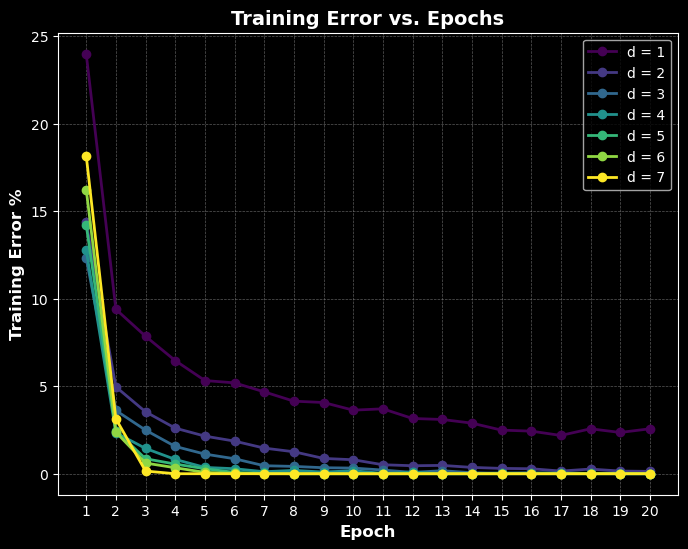
\includegraphics[width=\linewidth]{images/training_error_vs_epoch.png}
        \caption{Training Error vs Epoch}
        \label{fig:training-error}
    \end{subfigure}
    \hfill
    \begin{subfigure}[b]{0.45\linewidth}
        \centering
        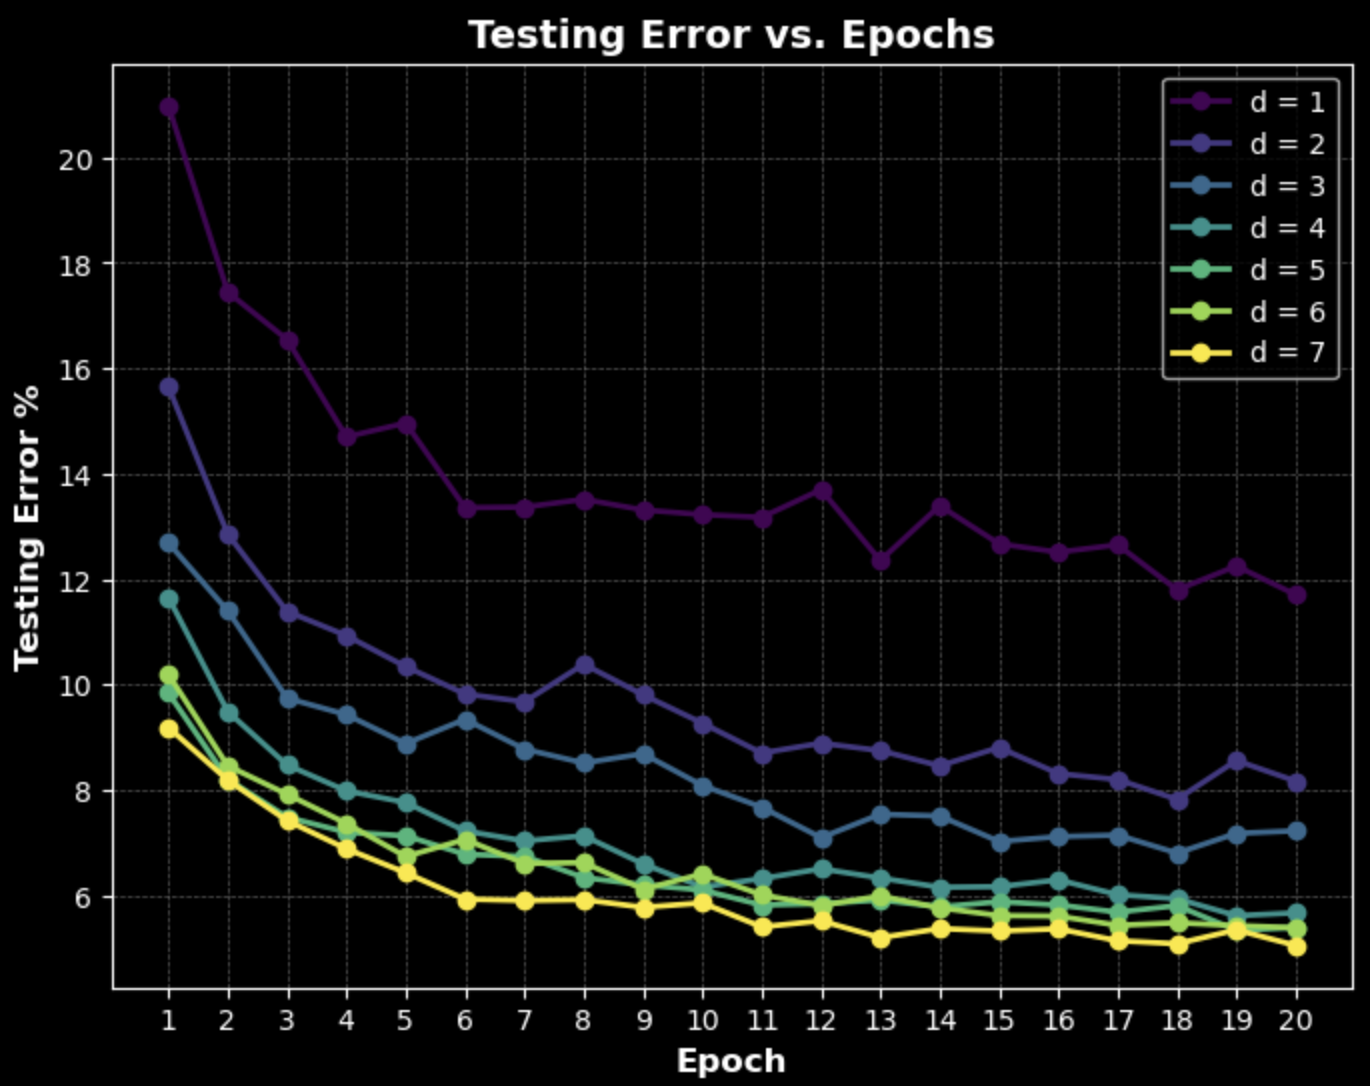
\includegraphics[width=\linewidth]{images/testing_error_vs_epoch.png}
        \caption{Testing Error vs Epoch}
        \label{fig:testing-error}
    \end{subfigure}
    \label{fig:side-by-side}
\end{figure}

From the graphs, we chose the number of epochs to be 13, as it seems to be where the errors start to converge. 

\subsection{}

We evaluate the performance of a classification model using the polynomial kernel across our range of parameter values. For each parameter, the dataset is repeatedly split into training and testing subsets, and the model is trained and evaluated 20 times. Training and testing errors are calculated for each split, and their mean and standard deviation are computed. These results are shown in the table below: 

\begin{table}[H]
\centering
\caption{Training and testing errors for different values of $d$}
\begin{tabular}{cccc}
\toprule
$d$ & Training (\%) & Testing (\%) \\
\midrule
1.0 & $3.75 \pm 0.88$ & $5.98 \pm 10.84$ \\
2.0 & $0.89 \pm 0.59$ & $2.65 \pm 1.68$ \\
3.0 & $0.42 \pm 0.14$ & $2.31 \pm 1.01$ \\
4.0 & $0.03 \pm 0.07$ & $2.01 \pm 1.31$ \\
5.0 & $0.01 \pm 0.00$ & $2.94 \pm 1.88$ \\
6.0 & $0.00 \pm 0.00$ & $3.23 \pm 1.95$ \\
7.0 & $0.00 \pm 0.00$ & $3.79 \pm 2.89$ \\
\bottomrule
\end{tabular}
\end{table}

From the table, we see that the optimal value for the parameter $d$ should be between $3.0$ and $5.0$. 

\subsection{}

We evaluate the classification model using cross-validation with polynomial kernels to optimize $d$. The dataset is repeatedly split into training and validation subsets, and the model is trained and tested across different parameter values to minimize validation error. After selecting the optimal parameter, the model is retrained on the full training data and tested on a separate hold-out set to assess its performance. We repeat this process 20 times to calculate the averages and standard deviations of test errors, training errors and the parameter $d$, which are displayed in the table below:

\begin{table}[H]
\centering
\caption{Best $d^*$ and associated errors}
\begin{tabular}{ccc}
\toprule
Best $d^*$ & Train Error & Test Error \\
\midrule
$3.85 \pm 0.67$ & $0.11 \pm 0.30\%$ & $1.92 \pm 1.10\%$ \\
\bottomrule
\end{tabular}
\end{table}

We find that the optimal value for $d$ is $d^*=3.85$, which falls into the range described in the previous question. 

\subsection{}
To evaluate the classification model's performance, we print its confusion matrix. For each test, we track how often each true digit is misclassified as another, compiling this data across 20 runs. These matrices are normalized into error rates based on digit frequencies then averaged. The results displayed as a heatmap show us the model's strengths and weaknesses. 
\begin{figure}[H]
    \centering
    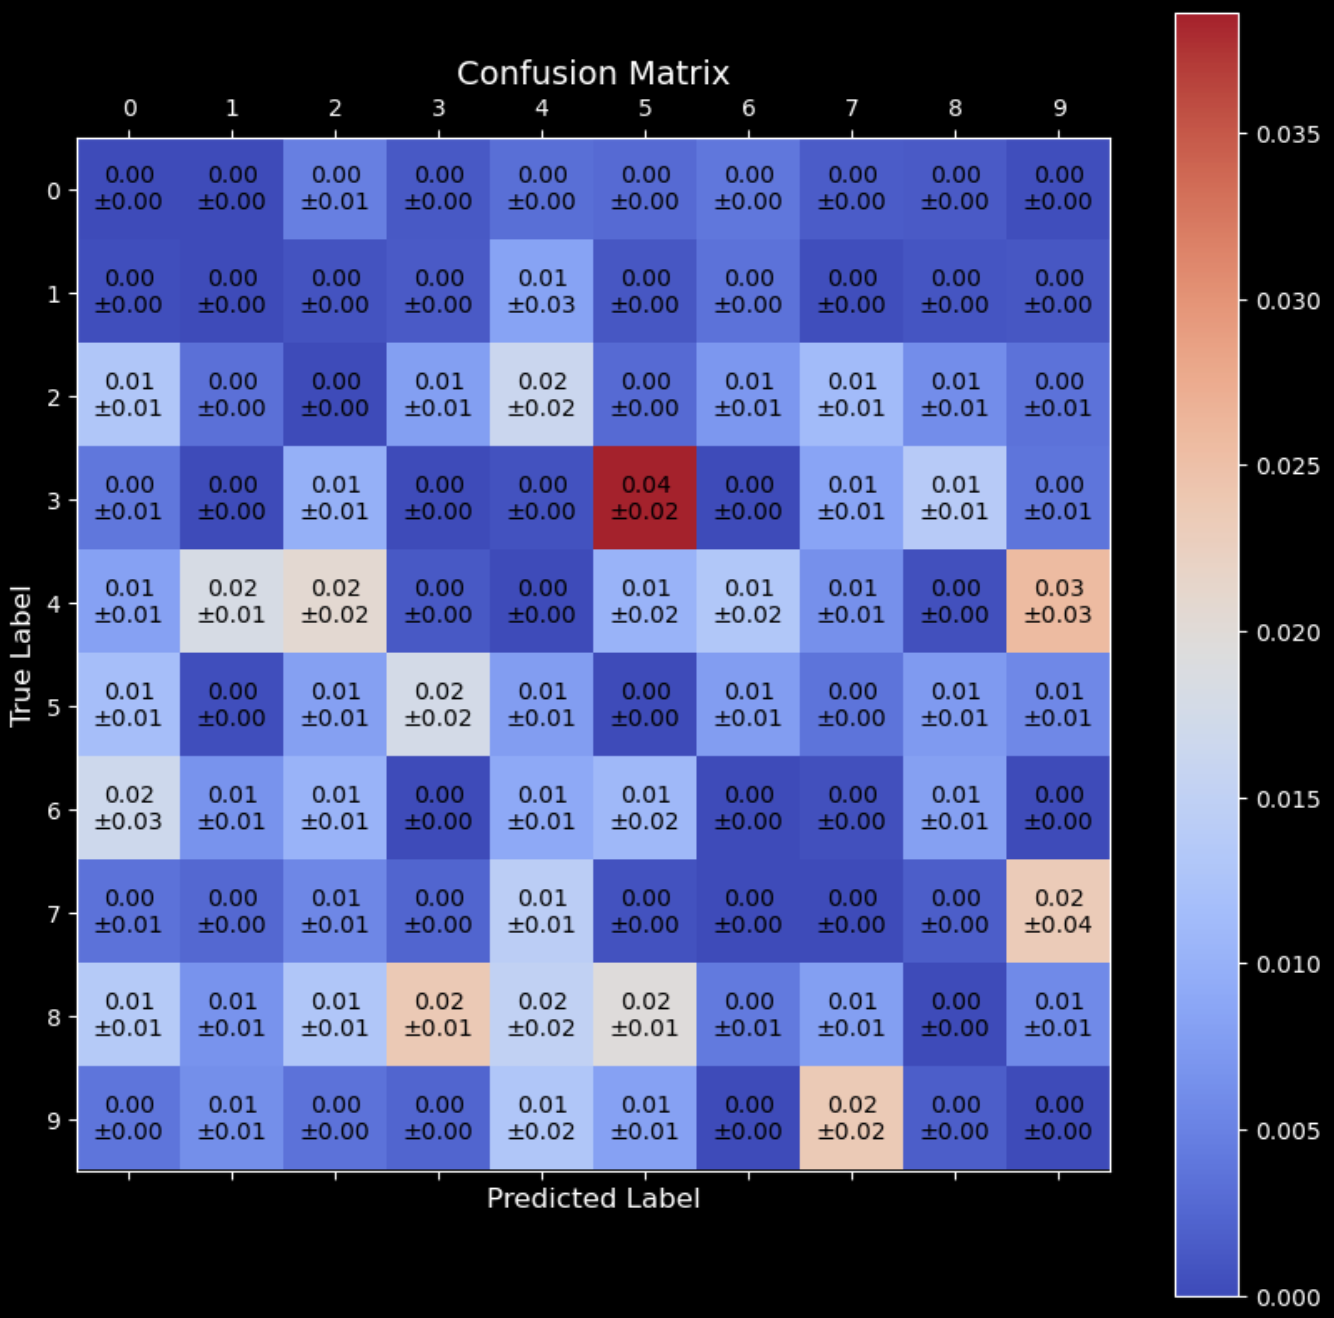
\includegraphics[width=0.8\linewidth]{images/confusion_matrix.png}
    \caption{Figure showing the confusion matrix of the classifier}
    \label{fig:confusion_matrix}
\end{figure}

From figure \ref{fig:confusion_matrix}, we notice that the model struggles to distinguish between a 3 and a 5, as it has the highest error rate of approximately $0.04$. It also struggles to distinguish between a $9$ and a $4$, as it has an error rate of around $0.03$. The heatmap also shows us that the model is good at identifying the digits $0$ and $1$. 

\subsection{}

We identified the hardest-to-classify images by repeatedly evaluating the model and isolating instances where its predictions differed from the true labels. Misclassified images and their labels were collected across multiple runs, making patterns of frequent errors emerge. The five most commonly misclassified images were then identified, and are displayed below, along with their true labels. 

\begin{figure}[H] % Use [H] to force placement, or [htbp] for more flexibility
    \centering
    \scalebox{0.8}{ % Scale down the entire figure group
        \begin{minipage}{\linewidth}
            \begin{subfigure}[b]{0.3\linewidth} % Reduce individual image size
                \centering
                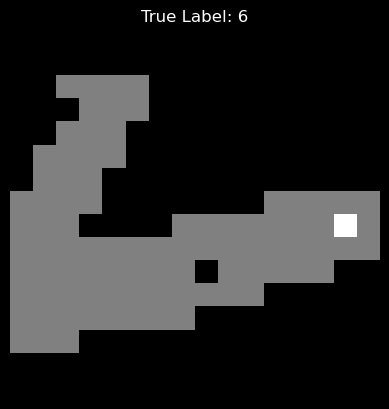
\includegraphics[width=\linewidth]{images/image_1.png}
                \caption{Image 1}
                \label{fig:image1}
            \end{subfigure}
            \hfill
            \begin{subfigure}[b]{0.3\linewidth}
                \centering
                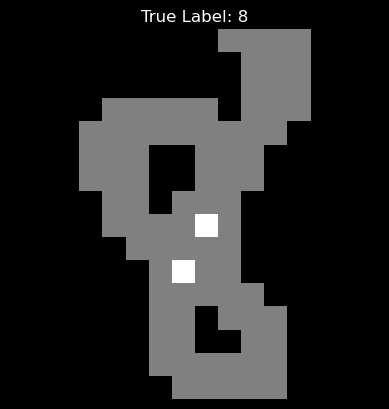
\includegraphics[width=\linewidth]{images/image_2.png}
                \caption{Image 2}
                \label{fig:image2}
            \end{subfigure}
            \hfill
            \begin{subfigure}[b]{0.3\linewidth}
                \centering
                
\includegraphics[width=\linewidth]{images/image_3.png}
                \caption{Image 3}
                \label{fig:image3}
            \end{subfigure}

            \vspace{0.3cm} % Reduce vertical spacing
            \begin{subfigure}[b]{0.3\linewidth}
                \centering
                
\includegraphics[width=\linewidth]{images/image_4.png}
                \caption{Image 4}
                \label{fig:image4}
            \end{subfigure}
            \hfill
            \begin{subfigure}[b]{0.3\linewidth}
                \centering
                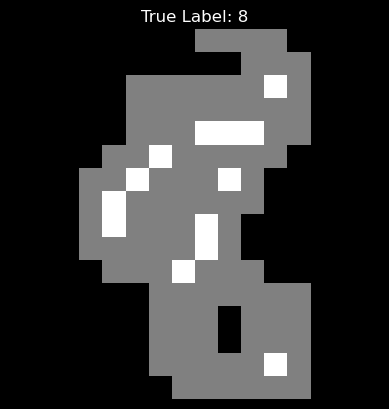
\includegraphics[width=\linewidth]{images/image_5.png}
                \caption{Image 5}
                \label{fig:image5}
            \end{subfigure}
        \end{minipage}
    }
    \caption{Figure showing the 5 most misclassified images}
    \label{fig:all-images}
\end{figure}

It is not surprising that these were hard to predict, as some would be ambiguous even for a human. Looking at Image 1 first, the 6 is very stretched out and almost looks like a 2. The other images also have some noise to them which would make them hard to predict: both the second and the third image have additional strokes (on the top right of both images) which could make it hard for the model to predict them. Image 4 is also ambiguous, looking like a 0, a 5 or 6. 

\subsection{}
\subsubsection{}

We chose the set of values for the parameter $c$ by using the coarse and fine search approach. To decide what the coarse search values should be, we consider the significance of the parameter. $c$ represents the width of the kernel (and being equivalent to $1/\sigma^2$), so it is positive. Thus we try a list of values between $0$ and $1$, and find the minimum testing error for each of them. The results are shown in Table \ref{tab:7a}:

\begin{table}[H]
\centering
\caption{Summary of Mean Errors with Std Deviation (RBF Kernel)}
\label{tab:7a}
\begin{tabular}{>{\centering\arraybackslash}p{2cm} >{\centering\arraybackslash}p{4cm} >{\centering\arraybackslash}p{4cm}}
\toprule
\textbf{c} & \textbf{Training Error (\%)} & \textbf{Testing Error (\%)} \\
\midrule
0.000001 & $64.90 \pm 2.94$ & $66.10 \pm 8.40$ \\
0.000005 & $63.50 \pm 2.30$ & $67.20 \pm 10.60$ \\
0.00001  & $64.10 \pm 2.60$ & $65.70 \pm 9.50$ \\
0.00005  & $59.80 \pm 7.60$ & $57.50 \pm 14.00$ \\
0.0001   & $48.50 \pm 12.60$ & $47.20 \pm 17.40$ \\
0.0005   & $28.00 \pm 7.60$  & $29.50 \pm 19.50$ \\
0.0010   & $14.00 \pm 2.40$  & $11.50 \pm 8.70$ \\
0.0050   & $2.30 \pm 1.00$   & $4.00 \pm 2.50$ \\
0.0100   & $0.40 \pm 0.30$   & $2.10 \pm 1.40$ \\
0.0500   & $0.00 \pm 0.00$   & $3.20 \pm 3.20$ \\
0.1000   & $0.00 \pm 0.00$   & $3.90 \pm 2.70$ \\
1.0000   & $0.00 \pm 0.00$   & $4.90 \pm 1.80$ \\
\bottomrule
\end{tabular}
\end{table}

From the table above, we can see that an optimal value for $c$ is between $0.005$ and $0.05$. We then proceed to a finer search between those values, and the results are shown in the table \ref{tab:7a2}:

\begin{table}[H]
\centering
\caption{Summary of Mean Errors with Std Deviation (RBF Kernel)}
\label{tab:7a2}
\begin{tabular}{>{\centering\arraybackslash}p{2cm} >{\centering\arraybackslash}p{4cm} >{\centering\arraybackslash}p{4cm}}
\toprule
\textbf{c} & \textbf{Training Error (\%)} & \textbf{Testing Error (\%)} \\
\midrule
0.0050 & $1.60 \pm 0.70$ & $3.00 \pm 2.50$ \\
0.0100 & $0.20 \pm 0.10$ & $1.80 \pm 1.40$ \\
0.0150 & $0.10 \pm 0.10$ & $2.10 \pm 1.20$ \\
0.0200 & $0.00 \pm 0.00$ & $2.40 \pm 2.00$ \\
0.0250 & $0.00 \pm 0.00$ & $3.80 \pm 2.70$ \\
0.0300 & $0.00 \pm 0.00$ & $5.90 \pm 3.60$ \\
0.0350 & $0.00 \pm 0.00$ & $6.40 \pm 3.85$ \\
0.0400 & $0.00 \pm 0.00$ & $7.20 \pm 3.20$ \\
0.0450 & $0.00 \pm 0.00$ & $6.70 \pm 3.30$ \\
0.0500 & $0.00 \pm 0.00$ & $7.10 \pm 3.90$ \\
\bottomrule
\end{tabular}
\end{table}


From the table above, we see that our lowest testing error is around $c=0.01$. For the rest of this question, we will use a range of 7 values (to match what was done for the polynomial) centered on $c=0.01$. 

\subsubsection{}

Running the question 3 procedure using the $S$ values for the parameters $c$ yields Table \ref{tab:7b}:

\begin{table}[H]
\centering
\caption{Summary of Mean Errors with Std Deviation (RBF Kernel)}
\label{tab:7b}
\begin{tabular}{cccc}
\toprule
\textbf{c} & \textbf{Training Error (\%)} & \textbf{Testing Error (\%)} \\
\midrule
0.0040 & 3.17 $\pm$ 1.35 & 3.71 $\pm$ 2.60 \\
0.0060 & 0.72 $\pm$ 0.68 & 2.50 $\pm$ 2.16 \\
0.0080 & 0.03 $\pm$ 0.09 & 1.98 $\pm$ 1.29 \\
0.0100 & 0.01 $\pm$ 0.03 & 1.14 $\pm$ 1.43 \\
0.0120 & 0.00 $\pm$ 0.00 & 1.97 $\pm$ 1.67 \\
0.0140 & 0.00 $\pm$ 0.00 & 1.29 $\pm$ 1.20 \\
0.0160 & 0.00 $\pm$ 0.00 & 1.26 $\pm$ 1.60 \\
\bottomrule
\end{tabular}
\end{table}

\subsubsection{}

Similarly, we run the question 4 procedure using the $S$ values for the parameters $c$ yields Table \ref{tab:metrics_c}:

\begin{table}[H]
\centering
\begin{tabular}{@{}lll@{}}
\toprule
\textbf{Best $c^*$} & \textbf{Train Error (\%)} & \textbf{Test Error (\%)} \\ \midrule
$0.0112 \pm 0.0037$     & $0.02 \pm 0.08$          & $2.12 \pm 1.63$          \\ \bottomrule
\end{tabular}
\caption{Performance Metrics}
\label{tab:metrics_c}
\end{table}

\subsubsection{}

We can see from the previous question that the Gaussian kernel outperforms the polynomial kernel. This could be due to the fact that the Gaussian kernel can model complex, nonlinear decision boundaries by mapping data to an infinite-dimensional space, unlike the polynomial kernel. Additionally, the Gaussian kernel is a radial basis function, which can help differentiate digits that have similar overall structures but vary in fine details. We can note however that this improvement comes at the cost of computational runtime. 

\subsection{}
\subsubsection{}

The One-versus-One (OvO) method, similarly to One-versus-Rest, is a technique used in multi-class classification tasks, but differentiates itself from OvR in the way it decomposes a multi-class classification problems. In OvO, each classifier distinguishes between a pair of classes: for a dataset with \( N \) classes, \( \binom{N}{2} = \frac{N(N-1)}{2} \) binary classifiers are created, where each classifier is trained on data from two specific classes and ignores the rest of the classes. To illustrate this, if we had three classes $C_1, C_2$ and $C_3$, we would need to train three classifiers: one to distinguish between $C_1$ and $C_2$, one to distinguish between $C_1$ and $C_3$, and one to distinguish between $C_2$ and $C_3$. In training, only the samples belonging to the two selected classes are used, which reduces the training data size for each classifier, making this method more computationally efficient that OvR for large datasets. When making predictions, each of the binary classifiers "votes" for one of the two classes it was trained to distinguish. The final predicted class is determined by this voting scheme, typically selecting the class with the most votes (majority voting).

\subsubsection{}

Running the question 3 procedure using the $S$ values for the parameters $c$ yields Table \ref{tab:8b}:

\begin{table}[H]
\centering
\caption{Summary of Mean Errors with Std Deviation (OvO)}
\label{tab:8b}
\begin{tabular}{>{\centering\arraybackslash}p{2cm} >{\centering\arraybackslash}p{4cm} >{\centering\arraybackslash}p{4cm}}
\toprule
\textbf{d} & \textbf{Training (\%)} & \textbf{Testing (\%)} \\
\midrule
1.00 & 1.63 $\pm$ 0.70 & 2.27 $\pm$ 2.27 \\
2.00 & 0.62 $\pm$ 0.31 & 1.21 $\pm$ 1.56 \\
3.00 & 0.04 $\pm$ 0.05 & 1.29 $\pm$ 1.46 \\
4.00 & 0.05 $\pm$ 0.04 & 1.44 $\pm$ 1.76 \\
5.00 & 0.05 $\pm$ 0.03 & 1.97 $\pm$ 1.45 \\
6.00 & 0.06 $\pm$ 0.03 & 1.76 $\pm$ 1.28 \\
7.00 & 0.05 $\pm$ 0.03 & 1.67 $\pm$ 1.35 \\
\bottomrule
\end{tabular}
\end{table}

\subsubsection{}

Similarly, we run the question 4 procedure using the $S$ values for the parameters $c$ yields Table \ref{tab:8c}:

\begin{table}[H]
\centering
\caption{Summary of Best Parameters and Errors}
\label{tab:8c}
\begin{tabular}{>{\centering\arraybackslash}p{3cm} >{\centering\arraybackslash}p{4cm} >{\centering\arraybackslash}p{4cm}}
\toprule
\textbf{Best $d^*$} & \textbf{Train Error (\%)} & \textbf{Test Error (\%)} \\
\midrule
3.00 $\pm$ 0.84 & 0.08 $\pm$ 0.23 & 1.52 $\pm$ 1.66 \\
\bottomrule
\end{tabular}
\end{table}

\subsubsection{}

Comparing the One-versus-Rest and the One-versus-One methods, we first notice that the optimal degree parameter is lower for OvO than for OvR. This could be due to the nature of the technique, as in OvO, each classifier only needs to distinguish between two classes, which generally requires simpler decision boundaries compared to OvR, where each classifier must distinguish one class from all others. On top of that, Each OvO classifier is trained on a subset of the data containing only the two relevant classes, making it less likely to require high model capacity ($d^*$) to fit the data. Secondly, we see that OvO has a lower test error than OvR. The One-versus-One pairwise classification reduces the complexity and might make the method more effective, as the model would be more tailored to resolving the overlap between two particular classes, (such as 3 vs 5, which we saw OvR had trouble distinguishing in the heatmap). 

\end{document}
